\documentclass[a4paper,12pt]{article}
\usepackage[dvipsnames]{xcolor}
\usepackage{etoolbox} \usepackage[english]{babel} \usepackage[utf8]{inputenc} \usepackage{amsmath} \usepackage{amsfonts} \usepackage{amsthm} \usepackage{graphicx} \usepackage[colorinlistoftodos]{todonotes} \usepackage{amsfonts} \usepackage{bbm} 
\usepackage{setspace} 
\usepackage{enumitem}
\usepackage{pdfsync} \usepackage{xr}
\usepackage[ruled]{algorithm2e}
\usepackage{tikz}
\usepackage{caption}
\usepackage{subcaption}
% \usepackage{authblk} % NEW!!!
% \bibliographystyle{econometrica}

\bibliographystyle{plainnat}
\usepackage{hyperref}       % hyperlinks
\hypersetup{
    colorlinks=True,
    citecolor=blue,
    linkcolor=blue,
    filecolor=blue,      
    urlcolor=blue,
    pdftitle={RFP},
    pdfpagemode=FullScreen,
    }

\usepackage{natbib}

\newtheorem{theorem}{Theorem}[section] \newtheorem{proposition}{Proposition}[section] \newtheorem{lemma}{Lemma}[section]

% \newtheorem{definition}{Definition}[section]
\newtheorem{example}{Example} \newtheorem{corollary}{Corollary}[section] \newtheorem{remark}{Remark}[section] \newtheorem{assumption}{Assumption} \newcommand{\citeposs}[1]{\citeauthor{#1}'s \citeyearpar{#1}} \newcommand\fnote[1]{\captionsetup{font=small}\caption*{#1}}

\def\qed{\rule{2mm}{2mm}} \parskip = 1.5ex
\textwidth 7in
\textheight 10 in
\oddsidemargin -0.4 in
\evensidemargin -0.4in
\topmargin -0.7in





\begin{document}


\begin{titlepage}
\title{A Deep Learning Assessment of the Right to Counsel}
%\shortTitle{Short title for running head}

\author{Patrick Power, Shomik Ghosh and Markus Schwedeler}
\date{\today}
\maketitle
\thispagestyle{empty} % makes the title page number not appear
\vspace{-2em}
\begin{abstract}
Drawing from the Deep Learning Literature and in the language of Category Theory, we introduce a simple and unified structure that generalizes ordinary least squares, allows for nonparametric cluster effects, and is inherently compositional, even under regularization. With this framework, we examine the effects of the Right to Counsel: a policy which ensures that low-income households facing eviction have access to free legal representation. Complimenting the existing Economic Literature on the topic, we consider the extent to which the policy makes it harder for low-income individuals to find housing. As some have suggested, if the Right to Counsel increases the cost of evicting a tenant, landlords might respond by making it more difficult to rent a unit in the first place. Exploiting the staggered roll-out of the policy across the state of Connecticut, our preliminary results suggest that certain subsets of the population may be adversely affected by the policy. 
\vspace{0.2in}\\
\noindent\textbf{Keywords:} Deep Learning, Evictions, Right to Counsel\\
%\noindent\textbf{JEL Codes:} key1, key2, key3\\
\end{abstract}
\setcounter{page}{1}
\end{titlepage}

%\thispagestyle{empty}

%\pagebreak \newpage


%\oneandhalfspacing
The paper can be decomposed into two main parts. In the first section, we introduce our empirical framework. In the second section, we apply this framework to better understand the consequences of the Right to Counsel. 
\section{Framework Introduction}
\subsection{Motivation}
Rarely is there a pre-established estimator that addresses most of the issues competing for ``first-order" importance in applied microeconomic studies. Data is  messy -- clusters of individuals receive the same treatment; people drop out of the sample; outcomes get censored; selection into treatment is unknown. Because of this, it can be helpful to have methods that are \textbf{well-targeted} (i.e. address a specific issue) and \textbf{composable} (i.e. the components fit together) so that researchers can adjust their models to their specific context. With this aim in mind, we illustrate that a regularized version of \cite{finn2017model} composed with a regularized neural ODE (\cite{kelly2020learning}) offers a conceptually simple way to adjust one's estimator for the presence of clustered data as well as to flexibly control the hypothesis space of the model. We highlight the usefulness of this approach both in terms of estimating nonparametric conditional expectation functions as well as low dimensional parameters of interest.
\subsection{Model}
In the language of Category theory, training the model is done in the Kleisi Category while inference occurs in the Category of Sets. Note for visual clarify we assume that composition of functions is of higher precedence than function application.\footnote{Expressing the framework in the language of category theory provides one with a clear way to understand the framework.}
\begin{align*} 
& \textrm{linearModel} \ \textcolor{blue}{\text{data}} \\
& \textrm{linearModel} \circ \ \textrm{identityMap} \ \textcolor{blue}{\text{data}} \\ 
& \textrm{linearModel} \circ  \big(\textrm{featureMap} \ \textcolor{blue}{\text{data}}\big) \ \textcolor{purple}{\text{params}} \\ 
& \textrm{linearModel} \circ  \big(\textrm{featureMap} \ \textcolor{blue}{\text{data}}\big) \circ \textrm{identityMap} \  \textcolor{purple}{\text{params}} \\ 
& \textrm{linearModel} \circ  \big(\textrm{featureMap} \ \textcolor{blue}{\text{data}}\big) \circ \big(\textrm{clusterMap} \ \textcolor{blue}{\text{data}}\big)  \textcolor{purple}{\text{params}} \\ 
& \textrm{linearModel} >=>  \big(\textrm{featureMap} \ \textcolor{blue}{\text{data}}\big) >=> \big(\textrm{clusterMap} \ \textcolor{blue}{\text{data}}\big)  \textcolor{purple}{\text{params}} \\ 
\end{align*}
\section{Problem}
\subsection{Context}
To keep things simple, we describe our approach in the specific context of cluster-level randomized control trials where we're interested in estimating treatment heterogeneity.\footnote{ Cluster-level randomized control trials are randomized control trials where treatment varies at a level above the unit of interest} Such experiments are common in development, education, and health settings because they are (A) generally easier to implement, (B) better adhere to the potential outcome framework\footnote{Reduce the chance of spillover effects between treated and non-treated individuals.} and perhaps most importantly\footnote{See John Lists's book, `The Voltage Effect` which highlights this importance in great detail} (C) allow us to understand the the effects of scaling the treatment.\footnote{Many large scale studies such as HIE prefer to include many control variables in their regression specification: size of family, age categories, education level, income, self-reported health status, and use of medical care in the year prior to the start of the experiment, kind of insurance (if any) the person had prior to the experiment, whether family members grew up in a city, suburb, or town, and spending on medical care and dental care prior to the experiment} With a binary treatment variable, such a problem can be decomposed into two separate problems where the objective function is minimized separately over the treatment and control groups.

\begin{align*}
    \underset{f \in \sigma(X)}{\text{inf}} \ E\big[(Y - f)^2\big]
\end{align*}
 

\subsection{Challenge (\textcolor{blue}{The Tragic Triad})\footnote{The expression "tragic triad" is taken from Gradient Surgery for Multi-Task Learning}}
Under the potential outcome framework, clustered level treatment assignment can be roughly thought of as forming the treatment and controls groups via random clustered sampling. From an estimation standpoint, this poses a few challenges because in each treatment group:
\begin{enumerate}
    \item We observe only a subset of the clusters
    \item The distribution of covariates can differ across clusters
    \item The distribution of outcomes conditional on covariates may differ across clusters
\end{enumerate}
The above issues are perhaps only magnified as we increase the dimensionality of the data. 
\begin{figure}[htbp]
\centering
\begin{subfigure}{.48\textwidth}
    \centering
    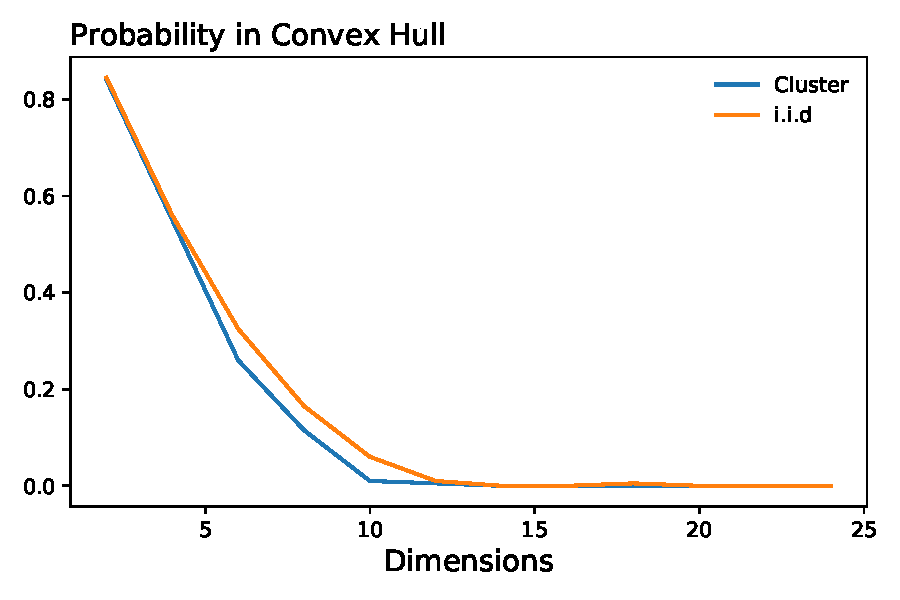
\includegraphics[width=.95\linewidth]{figures/framework/iid_cluster.pdf}
    %\caption{All zip codes}
    %\label{SUBFIGURE LABEL 3}
\end{subfigure}
\begin{subfigure}{.48\textwidth}
    \centering
    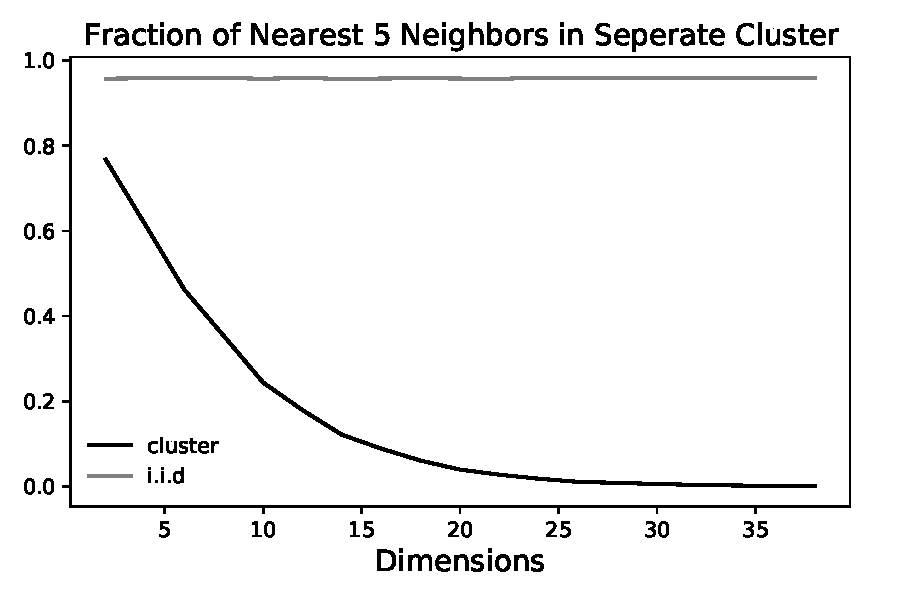
\includegraphics[width=.95\linewidth]{figures/framework/nearest_neighbors_increasing_correlation.pdf}
    %\caption{High Eviction Zip Codes}
    %\label{SUBFIGURE LABEL 4}
\end{subfigure}
%\caption{ \href{https://github.com/pharringtonp19/evictions/blob/main/scripts/cceh/primary/diff_n_mean_rrh.py}{Reproduced Here}: Confidence Bands formed via stratified bootstrapped sampling without replacement (75\%)}
%\label{FIGURE LABEL}
\end{figure}



The central challenge is how to incorporate a cluster indicator in the training phase so that the function adaptively pools information across clusters, without using the cluster indicator in the inference phase. To highlight this, we construct a toy data set where the average within cluster outcome value is zero (i.e. adding cluster specific fixed effects would not improve the fit to the data). The central challenge is how ``addaptively'' share information across clusters. That is, when there are a lot of clusters present, we would intuitively prefer a small bandwidth. When there are few clusters present, we would prefer a larger bandwidth. And of course, we would like to extend this to high dimensions.

\begin{figure}[htbp]
\centering
\begin{subfigure}{.48\textwidth}
    \centering
    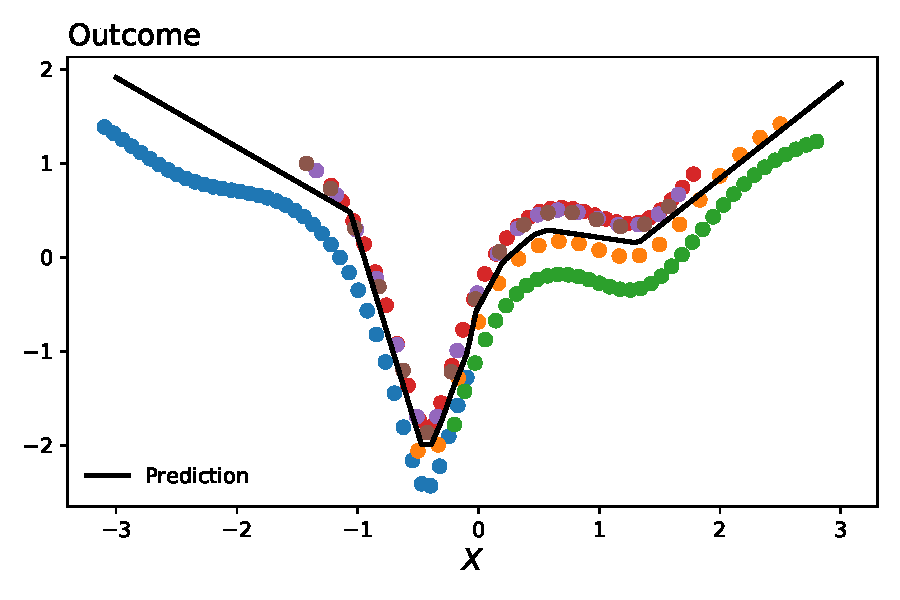
\includegraphics[width=.95\linewidth]{figures/framework/gradient_descent_motivating_example.pdf}
    %\caption{All zip codes}
    %\label{SUBFIGURE LABEL 3}
\end{subfigure}
\begin{subfigure}{.48\textwidth}
    \centering
    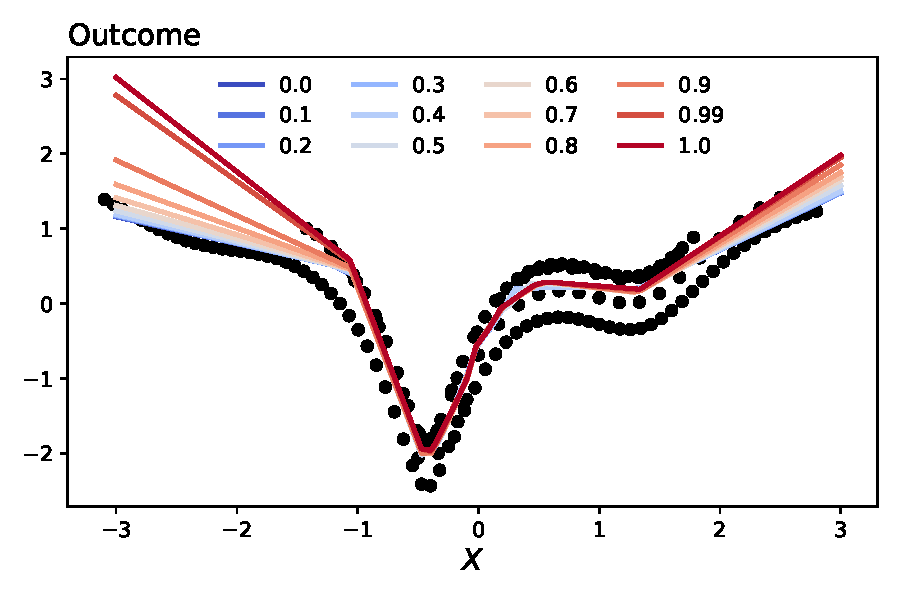
\includegraphics[width=.95\linewidth]{figures/framework/gradient_descent_motivating_example_tune.pdf}
    %\caption{High Eviction Zip Codes}
    %\label{SUBFIGURE LABEL 4}
\end{subfigure}
\caption{The general pattern that these figures try to highlight is that in order to fit the the `v`-shaped valley in the function, the model overfits the tails of the function -- \href{https://github.com/pharringtonp19/jmp_paper/blob/main/notebooks/gradient_descent_motivating_example.ipynb}{Reproduced Here}}
%\label{FIGURE LABEL}
\end{figure}
\section{Methodological Approach}

As applied microeconomists, we are accustomed to writing our problem as a bi-level optimization problem so as to better distinguish between the parameters of interest and the nuisance parameters. In this context, the nuisance parameters are cluster specific parameters that are ``fit'' during the inner optimization process. 
 
\begin{align*}
    \mathcal{L}(\theta) &:= \sum _c \mathcal{L}_c(\theta), \quad \mathcal{L}_c(\theta) := F(\theta, \theta^*_c(\theta)), \quad  \theta_c^*(\theta) := \underset{\theta_c}{\textrm{argmin}} \ F(\theta, \theta_c) 
\end{align*}
\begin{align*}
    \theta ^* &= \underset{\theta}{\textrm{argmin}}\ \mathcal{L}(\theta) \\ 
    &= \underset{\theta}{\textrm{argmin}}\ \sum _c \mathcal{L}_c(\theta)\\ 
    &= \underset{\theta}{\textrm{argmin}}\ \sum _c  F(\theta, \theta^*_c(\theta))\\
    &= \underset{\theta}{\textrm{argmin}}\ \sum _c  F(\theta, \underset{\theta_c}{\textrm{argmin}} \ F(\theta, \theta_c) )\\
\end{align*}
With “Classical” under-parameterized models, as in the case of linear regression, $F$, the clustere-specific empirical loss function is exactly what you would expect. 
\begin{align*}
    F(\theta, \theta_c^*(\theta)) := \sum _{i \in c}\big(y_i - \theta^Td_i - \theta _c^*(\theta)^Tx_i \big)^2
\end{align*}
 With“Modern” over-parameterized models, though, like the ones that we target in this paper, we make the following adjustments 
 \begin{enumerate}
     \item We restrict the objective function that is used to implicitly define the cluster specific maps. Without some form of augmentation/regularization, we can lose the learning signal as these models are capable of perfectly interpolating the data. 
     \item We generalize the above set-up by allowing the cluster specific parameters to be in one-to-one correspondance with the parameters of interest. 
     \item We add a penalty term to the cluster specific loss function to ensure that adaptation happens in the right space. 
 \end{enumerate}
 Taken together, these three points illustrate that approach is simply a regularized version of MAML. Although, as we highlight through extensive similations, the regularization part is key. 
 
 
\begin{align*}
    \hat{\theta}_c^*(\theta) &:= \underset{\theta_c}{\textrm{argmin}} \ G(\theta, \theta_c)  \\
    G(\theta, \theta_c)&= 
\end{align*}
Define our empirical cluster parameters in relation to the parameters of interest 
\begin{align*}
    F(\theta) := \sum _{i \in c}\big(y_i - f(\theta_c^*(\theta), x_i)\big)^2
\end{align*}
As well as introduce an auxilliary term to the cluster specific loss function: 
\begin{align*}
    \mathcal{L}_{c}(\theta) &= F(\theta) + H(\textrm{Path}(\theta, \hat{\theta}^*_c(\theta)))
\end{align*}

\begin{align*} 
&\text{regMAML} :: \text{Data} \rightarrow \text{Params} \rightarrow \big(\textrm{Params}, \text{Float}\big) \\
&\text{regMAML} \ \textcolor{blue}{\text{data}} \ \textcolor{purple}{\theta} := \Big(\text{Update}_m \circ \text{Update}_{m-1} \dots \circ \text{Update}_1 \Big) \ \textcolor{purple}{\theta}, \quad \mathcal{L}_c(\textcolor{blue}{\text{data}}, \textcolor{purple}{\theta})  \\ 
&  \quad \quad \quad \quad \quad \quad \quad \quad \quad \quad \text{where} \quad  \text{Update}_t \  \theta = \theta - \alpha_t \nabla \mathcal{L}_c(\textcolor{blue}{\text{data}}, \textcolor{purple}{\theta})
\end{align*}

\begin{align*}
    &\text{regNeuralODE} :: \text{Data} \rightarrow \text{Params} \rightarrow \big(\textrm{Data}, \text{Float}\big) \\
&\text{regNeuralODE} \ \_ \ \textcolor{blue}{x} \ \_ \ \textcolor{purple}{\theta} := x + \int f(t, x(t), \theta)dt, \quad \int \Big\| \frac{\partial ^k}{dt^k}f(t, x(t), \theta) \Big\|dt \\ 
& \quad \quad \quad \quad \quad \quad \quad \quad \quad \quad \text{where}  \quad x(0)=x \\ \\ 
\end{align*}
\begin{itemize}
    \item optimization based meta-learning algorithms
\end{itemize}
\begin{quote}
Model Agnostic Meta-Learning (MAML), a method that consists of two optimization loops, with the outer loop finding a meta-initialization,
from which the inner loop can efficiently learn new tasks.-- \cite{raghu2019rapid}
\end{quote}
\begin{quote}
    Does the meta-initialization learned by the
outer loop result in rapid learning on unseen test tasks (efficient but significant changes in the
representations) or is the success primarily due to feature reuse (with the meta-initialization already
providing high quality representations)? -- \cite{raghu2019rapid}
\end{quote}
\begin{quote}
    The results strongly support feature reuse as the predominant factor
behind MAML’s success-- \cite{raghu2019rapid}
\end{quote}
\begin{quote}
    We find that freezing even all four convolutional layers of the network (all layers except the network head) hardly
affects accuracy. This strongly supports the feature reuse hypothesis: layers don’t have to change rapidly at
adaptation time; they already contain good features from the meta-initialization.-- \cite{raghu2019rapid}
\end{quote}

\begin{figure}[htbp]
\centering
\begin{subfigure}{.32\textwidth}
    \centering
    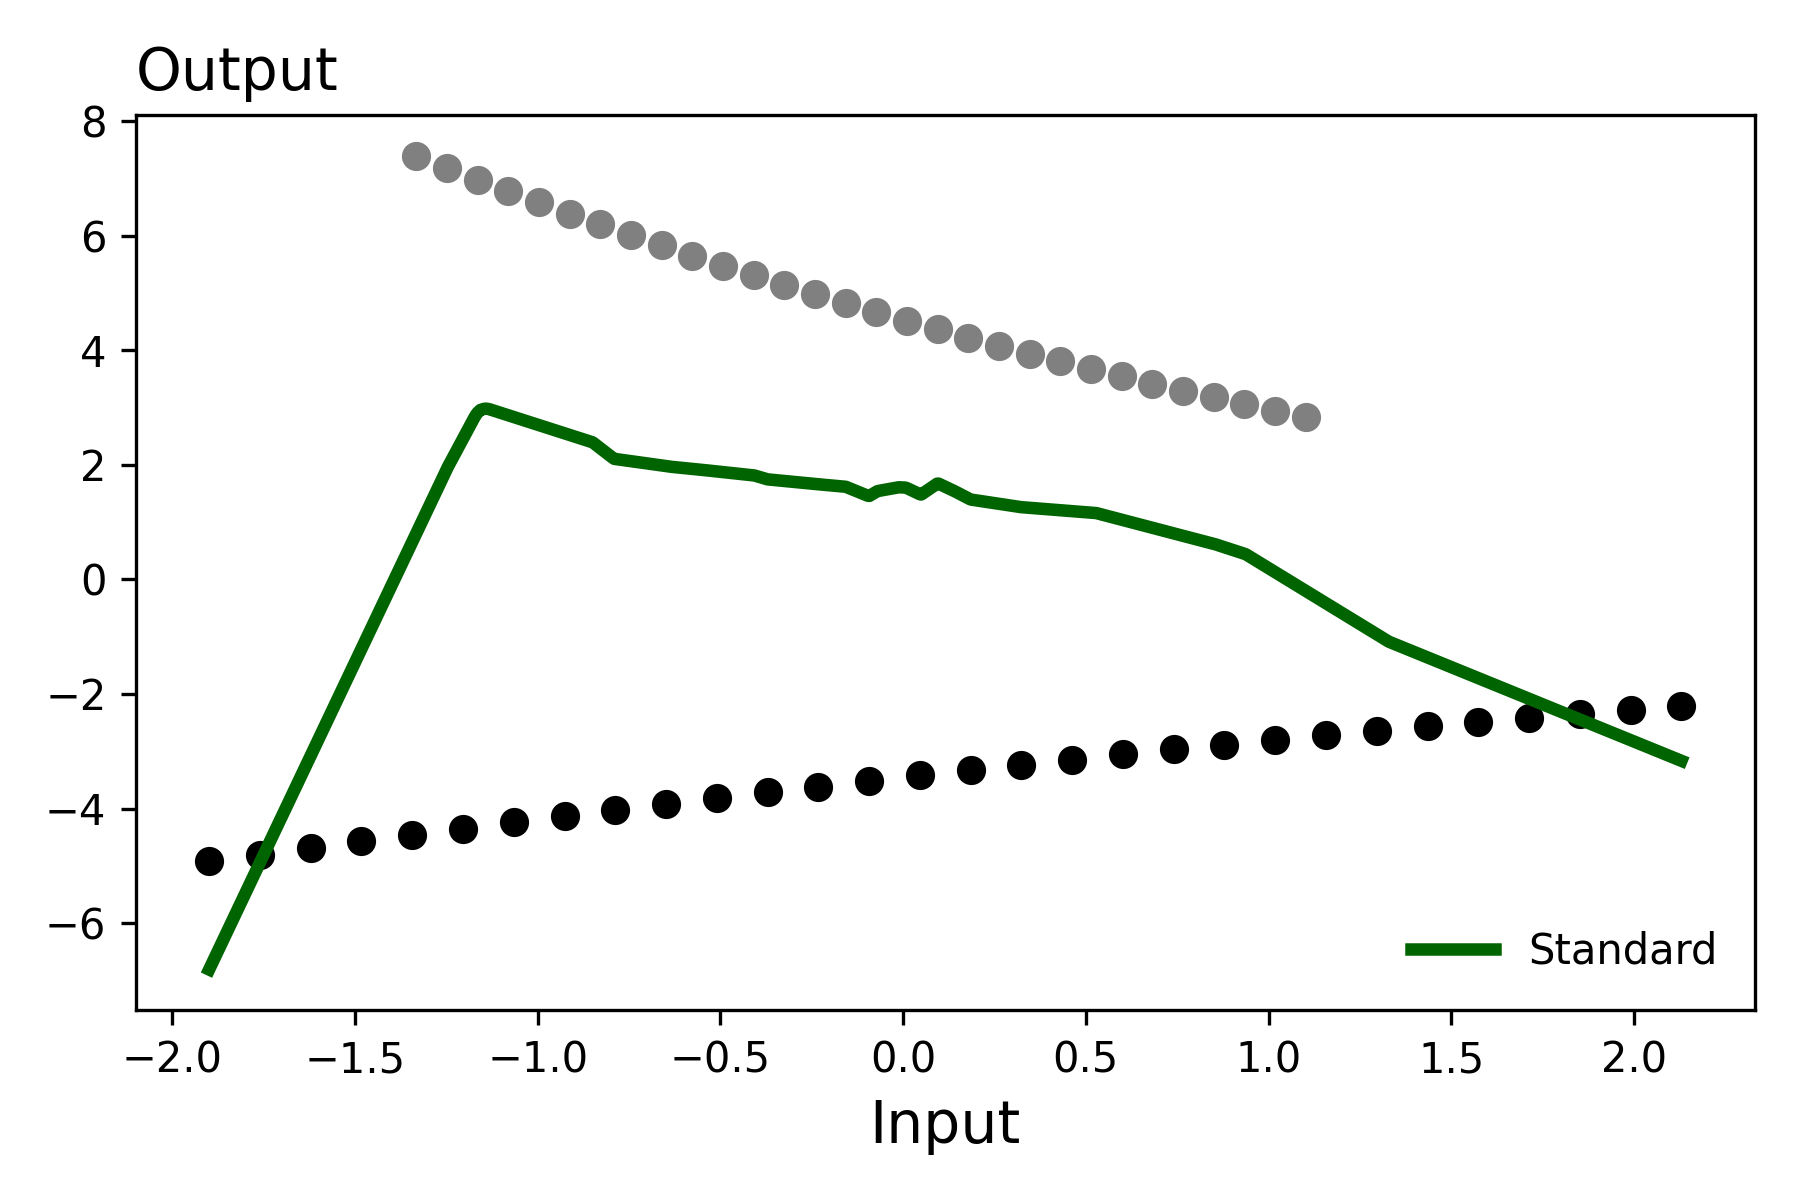
\includegraphics[width=.95\linewidth]{figures/framework/grad_desc_toy_Standard.png}
    \caption{Standard Training}
    %\label{SUBFIGURE LABEL 3}
\end{subfigure}
\begin{subfigure}{.32\textwidth}
    \centering
    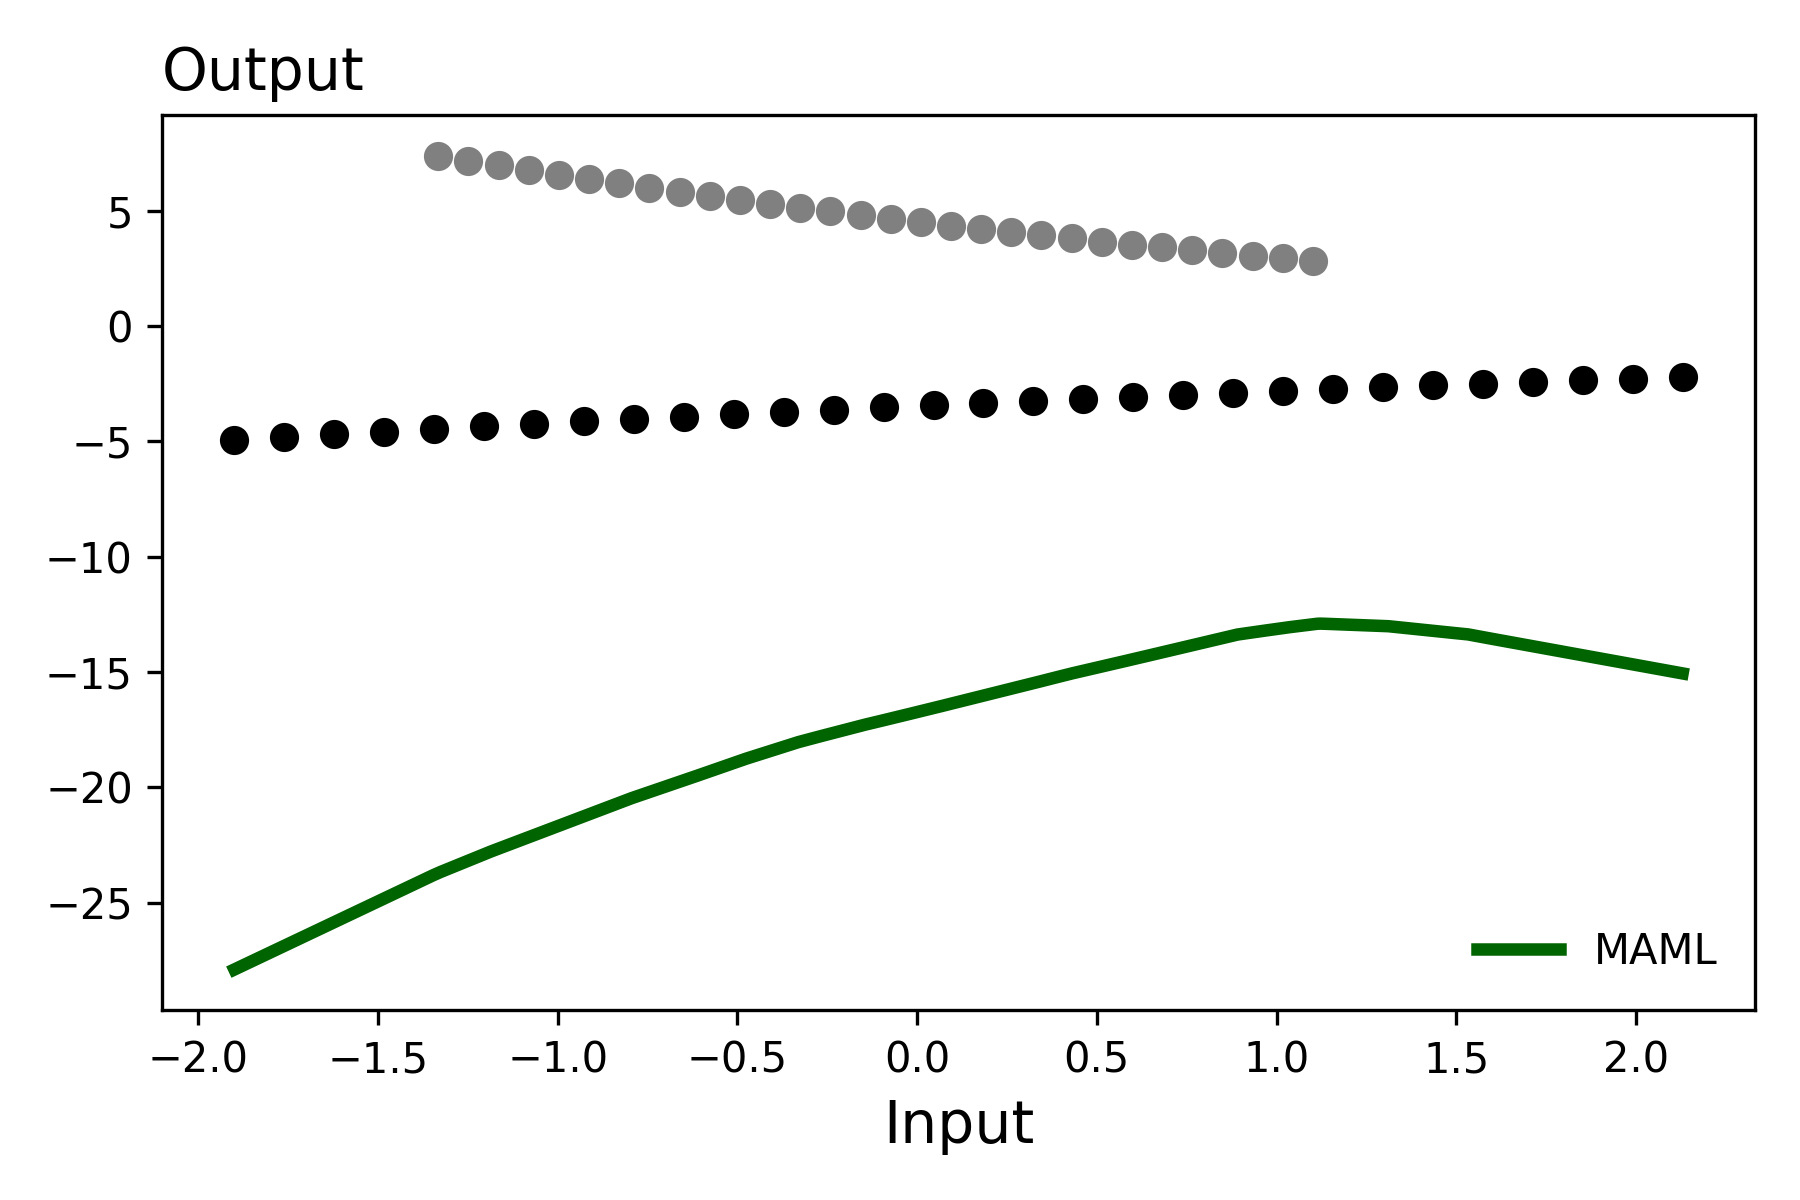
\includegraphics[width=.95\linewidth]{figures/framework/grad_desc_toy_MAML.png}
        \caption{MAML}
    %\label{SUBFIGURE LABEL 4}
\end{subfigure}
\begin{subfigure}{.32\textwidth}
    \centering
    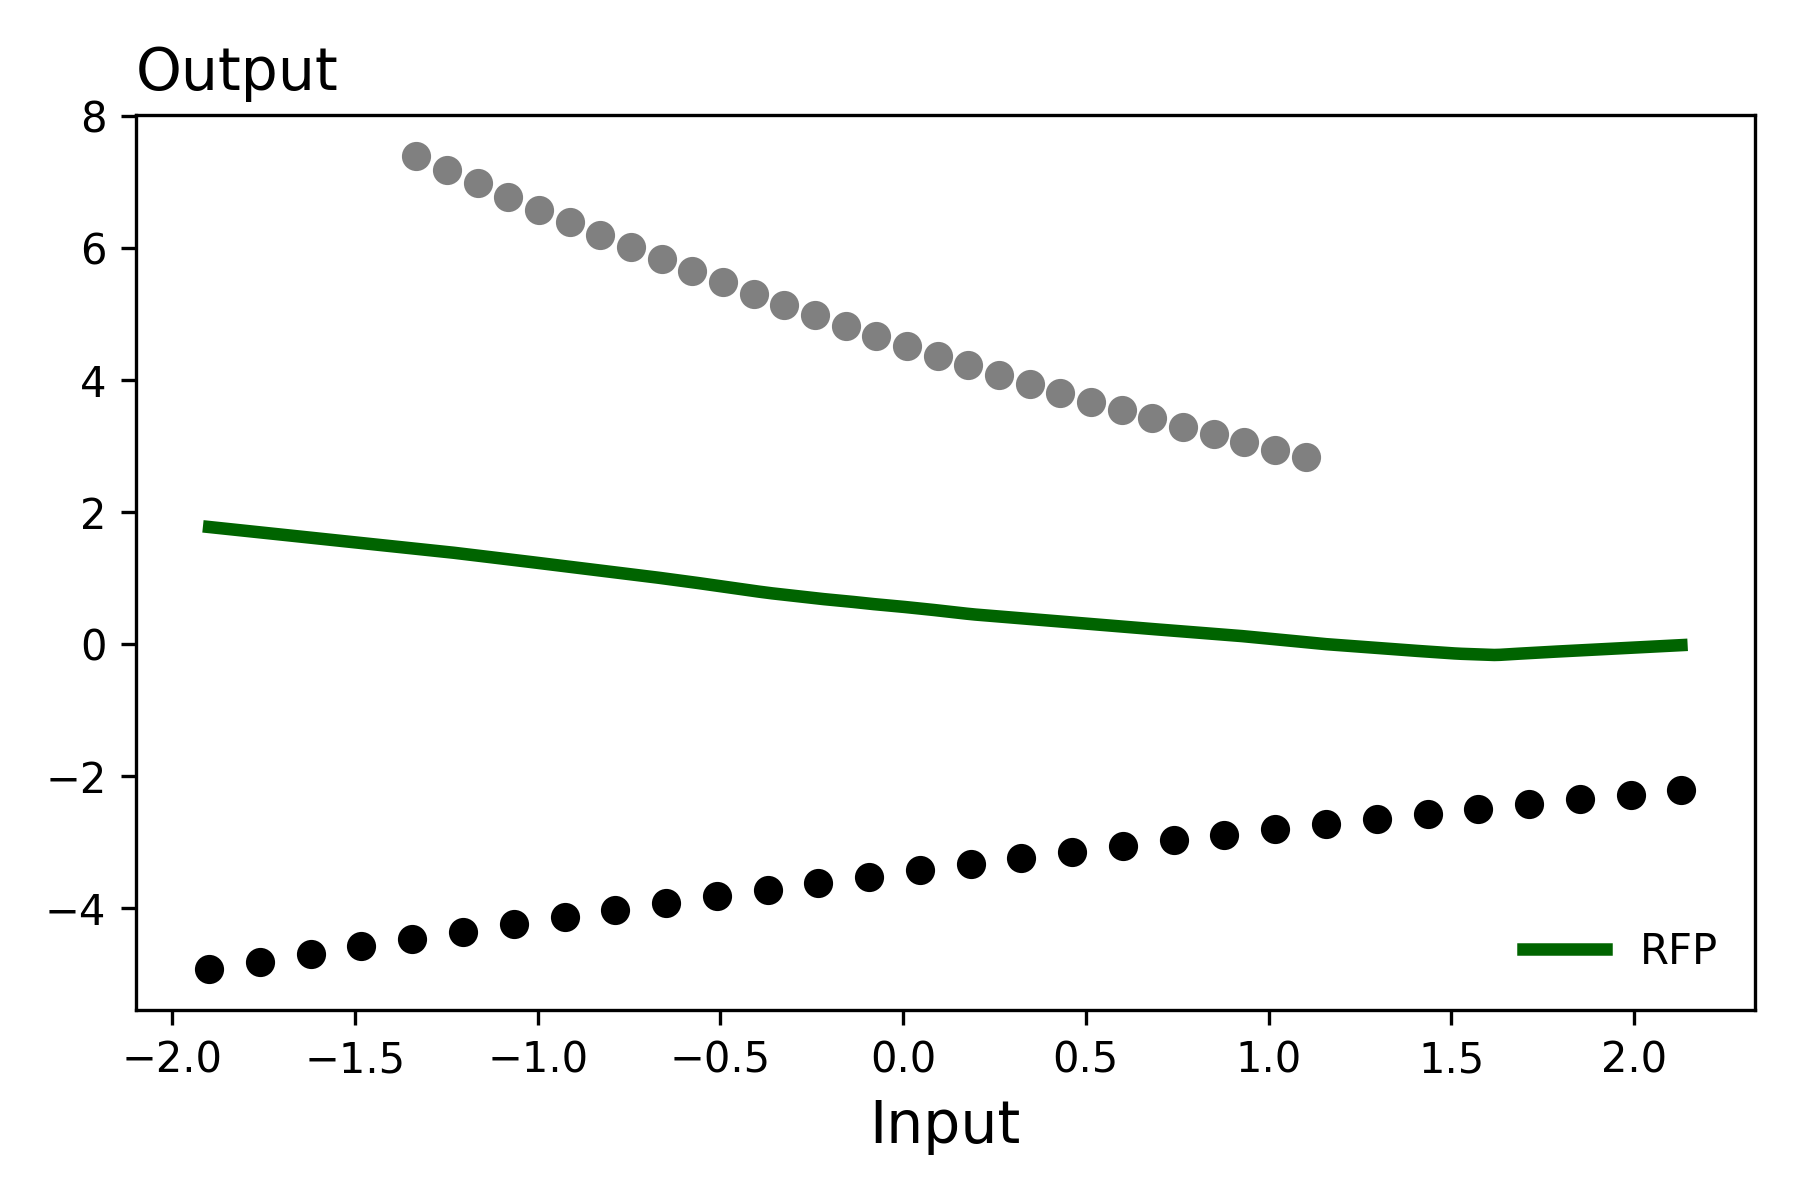
\includegraphics[width=.95\linewidth]{figures/framework/grad_desc_toy_RFP.png}
        \caption{RFP}
    %\label{SUBFIGURE LABEL 4}
\end{subfigure}
\caption{ \href{https://github.com/pharringtonp19/rfp/blob/main/notebooks/grad_desc_toy.ipynb}{Reproduced Here}: The grey and black dots represent data from separate clusters. Each figure corresponds to fitting a neural network to this data under different training algorithms}
\label{FIGURE LABEL}
\end{figure}
\section{Parametric Estimation}
What may not be clear from the above presentation is why this approach is useful for estimating finite parameters of interest. The thinking being that linear regression already partial out the cluster effect. In this context, though, when treatment varies at the level of the cluster, a cross-section regression with cluster level fixed effects 
\begin{figure}[htbp]
\centering
\begin{subfigure}{.48\textwidth}
    \centering
    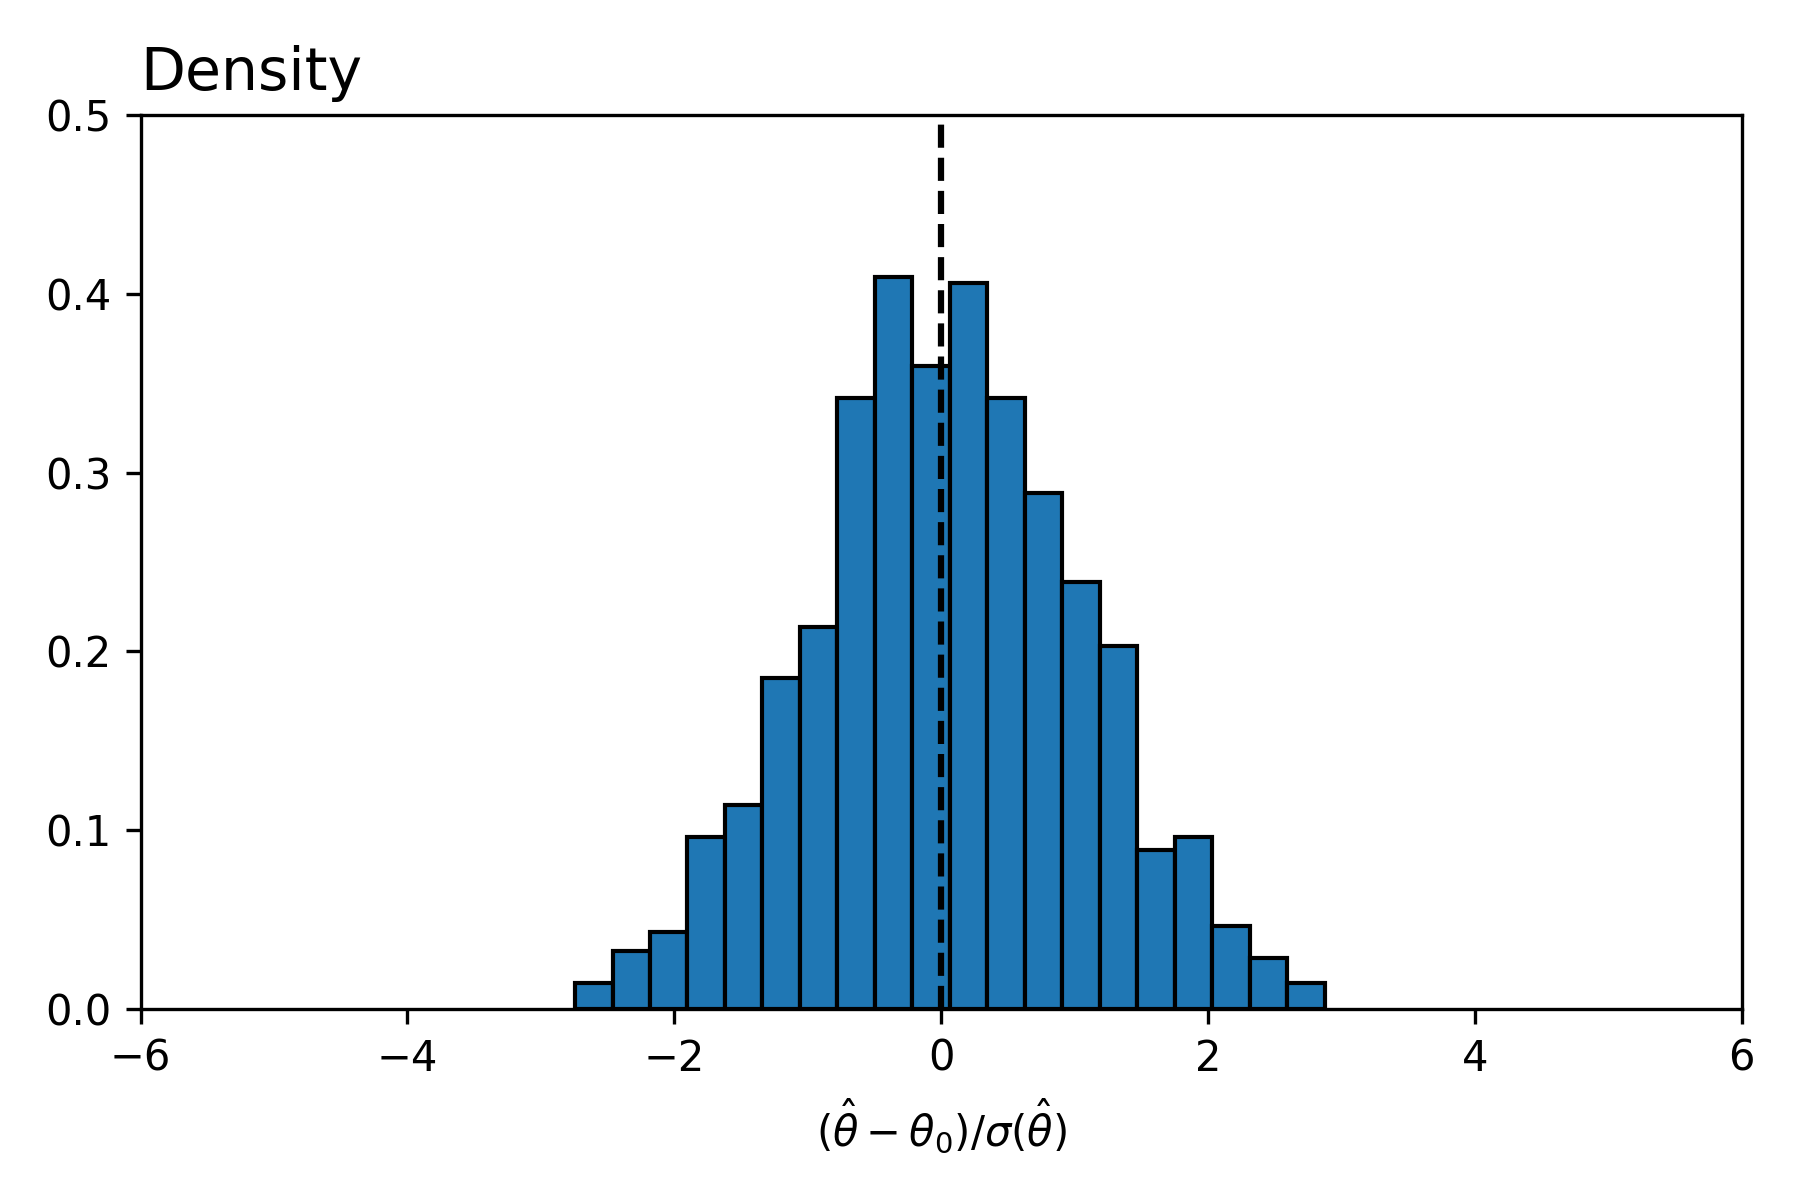
\includegraphics[width=.95\linewidth]{figures/framework/dml_True.png}
    \caption{Original Paper}
    %\label{SUBFIGURE LABEL 3}
\end{subfigure}
\begin{subfigure}{.48\textwidth}
    \centering
    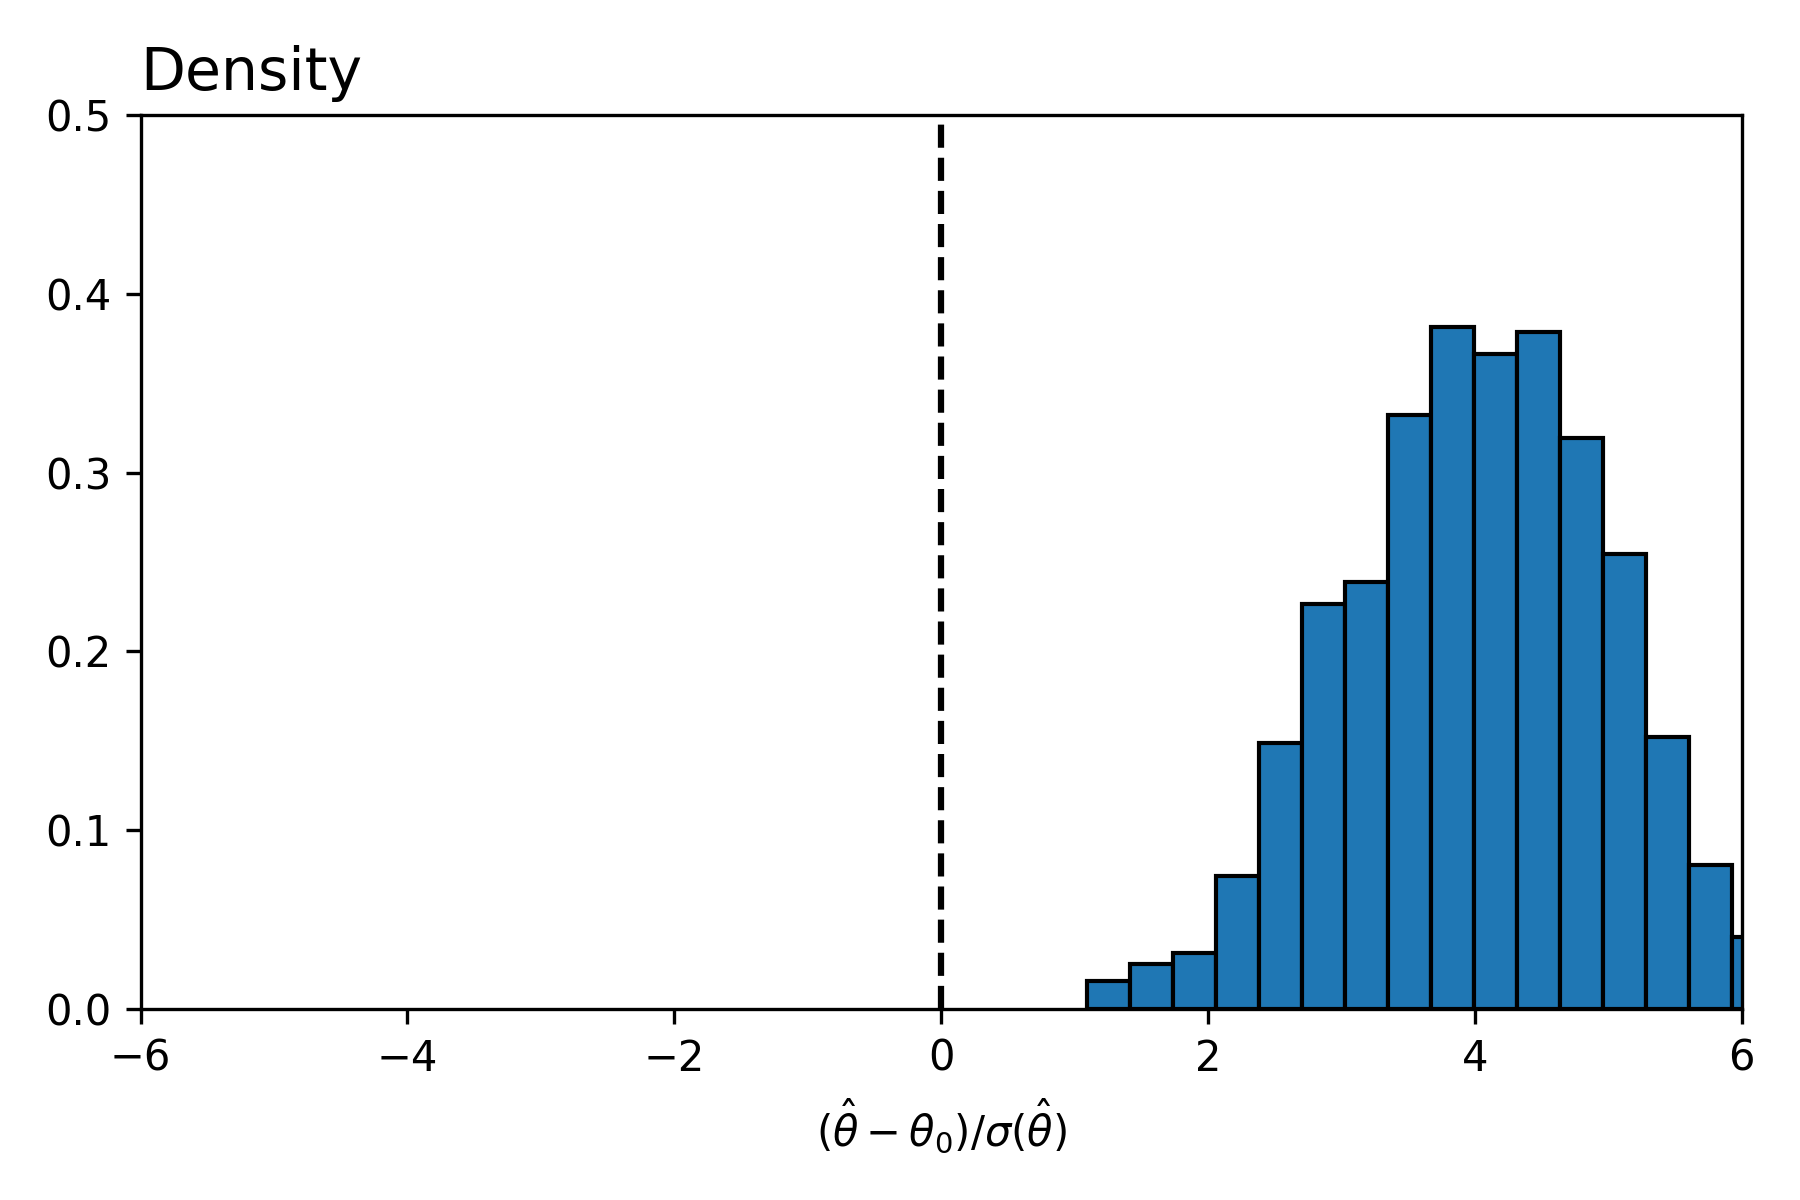
\includegraphics[width=.95\linewidth]{figures/framework/dml_False.png}
        \caption{Nonuniform Propensity Score}
    %\label{SUBFIGURE LABEL 4}
\end{subfigure}
\caption{ \href{https://github.com/pharringtonp19/rfp/blob/main/examples/scripts/dml.py}{Reproduced Here}: The sampling distribution of a Double Machine Learning Based Neural Network Estimator under selection on observables. }
\label{FIGURE LABEL}
\end{figure}
\section{Right to Counsel}
In this paper, the term \textit{The Right to Counsel} refers to a policy initiative which ensures that tenants have access to free legal representation in eviction cases. Unlike criminal cases in the U.S., defendants in an eviction case are not provided with a public attorney. A gap in legal representation therefore exists between landlords and tenants which \cite{collinson2022eviction} has documented to be as large as $95\%-1\%$ in some areas in favor of the landlord.
\subsection{Background \& Motivation}
The 2 million evictions that occur each year across the United States are costly to individuals, landlords, courts, and the general public.\footnote{Eviction number from \cite{gromis2022estimating}. (Individual Costs): \cite{collinson2022eviction} writes, ``We find that eviction causes significant disruptions that are reflected in increases in residential mobility, homelessness, and hospital use''. (Court Costs): As \cite{seron2001impact} notes, legal representation actually might decrease housing court costs as the number of appearances and post judgement motions decline. (General Public): As \cite{desmond2019unaffordable} writes, ``Residential instability often brings about other forms of instability—in families, schools, communities— compromising the life chances of adults and children''} Given the severity of these costs, the multitude of factors which contribute to an eviction filling, and the typical manner in which eviction cases are settled, many in the U.S. believe that free legal counsel should be provided to households facing eviction.\footnote{(Multitude of Causes):  David Ehrens writes in his \href{https://dartmouth.theweektoday.com/article/opinion-support-right-counsel-renters/58185}{letter} to the editor of \href{https://dartmouth.theweektoday.com/}{Dartmouth Week} of ``evictions related to the pandemic, chronic housing supply shortages, inequities in lending, generational poverty, and other harms''. (Eviction Proceedings): \textcolor{blue}{Missing Reference} writes ``the vast majority resolved by default or settlement, typically the result of hallway negotiation'' (Growing Interest): \cite{engler2010connecting} writes ``a renewed call for a civil right to counsel, or civil Gideon, has gained momentum \dots as well as a surge in membership in the newly-created National Coalition for a Civil Right to Counsel.''} And indeed, over the past five years, $15$ cities and $3$ states have acted on this belief, initiating a Right to Counsel in some form for low-income households, with additional localities starting pilot studies in the hope of closing the gap in legal representation and improving outcomes. \par 
To some extent, this hope has been empirically justified when looking at the direct legal outcomes of eviction cases. Both in the context of small scale randomized control trials as well as in city-wide roll-outs, researchers have generally found weakly positive to positive results with \cite{seron2001impact}  writing that ``Represented tenants are much less likely to have a final judgment and order of eviction against them'' and \cite{cassidy2022effects} reporting ``Tenants with lawyers are considerably less likely to be subject to possessory judgments, face smaller monetary damages, are less likely to have eviction warrants issued against them, and are ultimately less likely to be evicted.''\footnote{\cite{greiner2012limits} examines the outcomes of two small scale, Massachusetts based, randomized control trials and finds a measurable impact of legal representation in only one of the trials.} \par 
A natural concern, though, is that these legal results might be diminished or possibly out-weighted by the associated indirect effects that emerge when the policy is rolled out at scale. That is, when the policy covers a significant fraction of the population such that landlords are incentivized to respond, the net effect may differ substantially from the above reports. One of the most consistent findings in the literature to date is that legal services increase the duration of eviction proceedings. As voiced both in the academic literature as well as in personal conversations with lawyers, it seems likely that some of these costs will be passed on to low-income households, and perhaps in particular, to those who can least bear them.\footnote{(Academic Shifting Costs): \cite{gunn1995eviction} writes, ``By increasing landlords' costs of doing business, legal services attorneys may enrich their clients at the expense of all other similarly situated poor tenants." (Laywer Shifting Costs):  A lawyer who specializes in evictions wrote via email that `The thing to remember is that higher costs for landlords always get passed on to the tenants in some form (higher rent, deposits, fees, etc.), or the property gets sold, thereby reducing inventory and resulting in higher rents.''} Up to this point, though, there has been little to no empirical work on this highly relevant policy question. \par 
\subsection{Approach}
In order to motivate the specific approach of this paper, it is important to highlight why the above concern remains an open question. There are two closely related reasons for this. The first is that the data required to make an empirical assessment of the Right to Counsel at scale is relatively new. As recently as last year, the most attractive approach to answering this research question was via a counterfactual analysis as in \cite{abramson2021welfare}. The second reason is that the adverse effects of the Right to Counsel are likely difficult to measure. Given the informal nature of evictions, -- Mathew Desmond suggests in his New York Times Best Seller, \textit{Evicted}(\cite{desmond2016evicted}), that informal evictions account for $48\%$ of forced moves while formal evictions account for $24\%$ -- it seems reasonable to expect landlords to operate in some informal, or hard to detect way such as by asking for a higher security deposits, requiring additional months of rent upfront or increasing screening standards. It's not been clear, therefore, what type of data exists that might allow researchers to make even a partial assessment of these general equilibrium effects. \par 
This paper takes a ``noisy'' first step towards addressing both of these issues. First, it exploits the ongoing rollout of the policy across the state of Connecticut where, due to supply constraints of legal services, only low-income individuals in certain zip codes currently receive free legal aid. Second it makes use of data from the U.S. Department of Housing and Urban Development which measures both the characteristics of individuals experiencing homelessness (race, gender, family structure) as well as their length of their housing search. Importantly, this data set is restricted to households who don't face significant barriers to housing. That is, households who are thought to require only limited and partial support. The search length of these households (reflected in the \textcolor{blue}{blue} transition arrows in figure \ref{fig:1}) are therefore a key outcome variable for policy makers are likely a strong indication of whether there are adverse effects of the policy at scale. 

Lastly, while no pre-analysis plan accompanies this paper, the only source of heterogeneity explored is the effects of the policy on Black and female tenants. As well documented in the eviction literature, these subgroups share the greatest likelihood and costs of evictions, as \cite{desmond2019unaffordable} writes, ``Low-income women, especially poor black women, are at high risk of eviction'', and \cite{collinson2022eviction} notes that with regards to the costs of evictions, ``We find particularly sharp negative impacts for female and Black tenants, who drive the effects on labor market outcomes, residential mobility, and interactions with homelessness.'' It seems likely, therefore, that if landlords respond in an adverse way to The Right to Counsel, it would be be towards this sub-population in particular. Hence, all regression specifications are fit both over the entire sample and this sub-sample of interest.

\section{Policy Details}
\subsection{Timeline}
In June of 2021, Governor Lamont of Connecticut signed into law the Right to Counsel (3). As highlighted in the timeline below, this event coincides with the end of the local moratorium on evictions (4) in Connecticut. Six months later, on January 31, 2022, as Covid-19 relief was winding down, the Right to Counsel went into effect. A detailed description of the timeline is provided in the appendix, but key dates of interest, including the start and end of local and national moratoriums, are illustrated below. 
\par 
\begin{figure}[htbp]
\centering
    \centering
    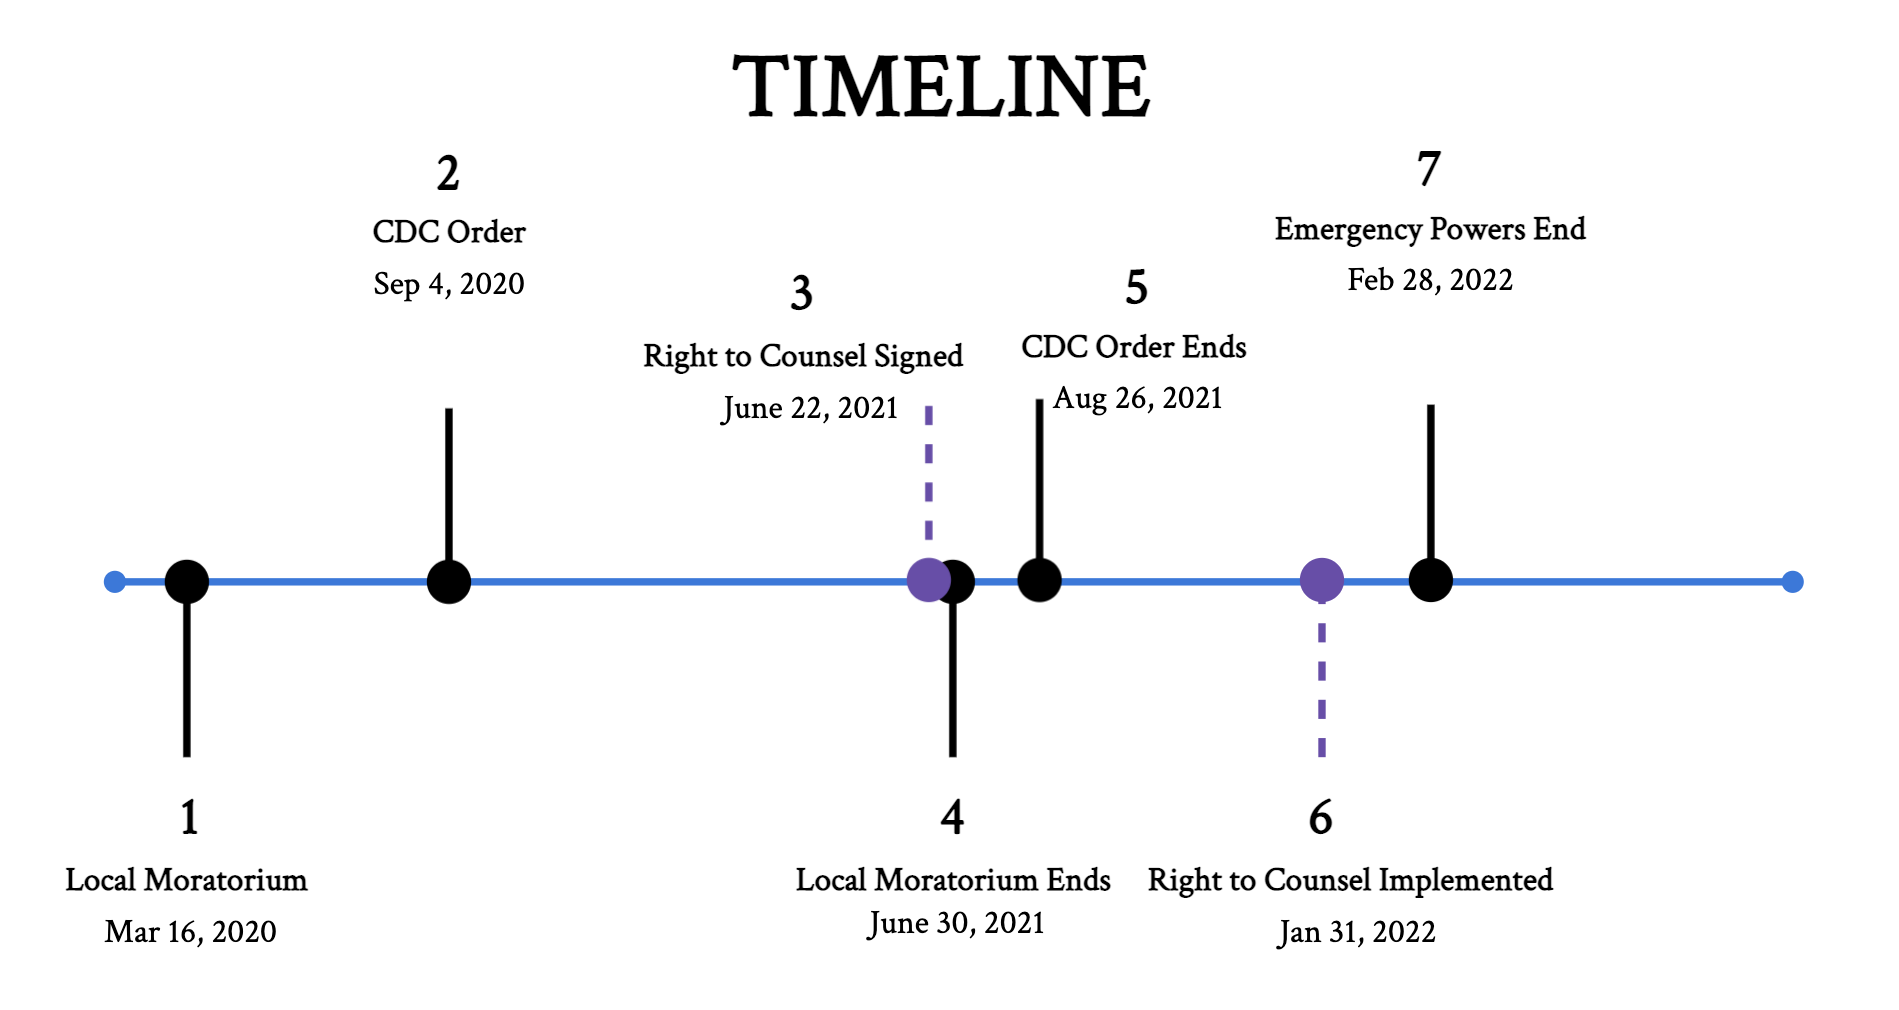
\includegraphics[width=.60\linewidth]{figures/rtc/context/timeline.png}
    %\caption{All zip codes}
    \label{SUBFIGURE LABEL 3}
\end{figure}

\subsection{Implementation}
Because the expected demand for legal services under the Right to Counsel exceed the current level of legal support, state representatives decided to implement the policy in phases.\footnote{During the two years leading up to the pandemic, Connecticut saw 20,000 eviction fillings on average\footnote{\href{https://youtu.be/sLpi4xlVGgU?t=1002}{link}}} In the first stage, the policy was made available to a subset of the zip codes (the 14 shown in yellow) which correspond to $30\%$ of evictions and $20\%$ percent of the renter population.\footnote{CBF Assignment Sheet-- received via email on August 26th --Expected to assist 2,000 households in the first phase, in a state where 20,000 residents faced eviction} Individuals and families within these zip codes who made $80\%$ or less than the area median income were eligible for legal support starting on January 31, 2022.\footnote{(\href{https://www.cga.ct.gov/2021/ACT/PA/PDF/2021PA-00034-R00HB-06531-PA.PDF}{"Income-eligible"} means (A) having household income at or below
eighty per cent of the state median income adjusted for family size, as
determined by the United States Department of Housing and Urban
Development, at the time of the request for representation; or (B)
receiving one of the following types of public assistance: (i) Temporary
Assistance for Needy Families, (ii) Supplemental Nutrition Assistance
Program benefits, (iii) Medicaid, (iv) Supplemental Security Income, (v)
refugee resettlement benefits, (vi) rental assistance under chapter 138a
of the general statutes, or (vii) the federal Housing Choice Voucher
Program, 42 USC 1437f(o); } Beginning earlier, on October 1, 2021, landlords were to notify individuals of the existence of this policy when serving tenants with a notice to quit (the first step in an eviction proceeding -- the entire process is described in more detail in the appendix). In addition to landlords, courts were expected to inform tenants of the policy when and if tenants appeared in court.\footnote{\href{https://www.cga.ct.gov/2021/ACT/PA/PDF/2021PA-00034-R00HB-06531-PA.PDF}{``On} and after October 1, 2021, an owner, lessor, landlord, legal
representative or agent of an owner, lessor or landlord, a housing
authority or a housing subsidy program administrator, as applicable,
shall attach a copy of the notice described under subdivision (1) of this
subsection, to (A) a notice to quit delivered to a covered individual
pursuant to chapter 832 or chapter 412 of the general statutes; (B) a
summons and complaint for a summary process action pursuant to
chapter 832 or chapter 412 of the general statutes; (C) a lease termination
notice for a public or subsidized housing unit; and (D) a notice to
terminate a state or federal housing subsidy''}\footnote{\href{https://www.cga.ct.gov/2021/ACT/PA/PDF/2021PA-00034-R00HB-06531-PA.PDF}{``An}y court notice scheduling a mediation or hearing that is sent to
a self-represented party in a covered matter shall include plain language
information about the availability of legal representation through the
right to counsel program and a phone number for accessing information
and applying for assistance.''} Given that the lack of enforcement with respect to landlords and that $37\%$ of Connecticut tenants fail to appear in court during eviction proceedings, it's quite possible that many eligible tenants are not yet aware of the policy's existence.\footnote{According to \href{https://www.ctpublic.org/news/2022-01-30/some-residents-facing-eviction-could-now-be-eligible-for-free-legal-aid}{article} $37\%$ of Connecticut tenants fail to appear in court during eviction proceedings, and their cases end in default, according to a 2021 report by the Connecticut Advisory Council on Housing Matters.}
\begin{figure}[htbp]
\centering
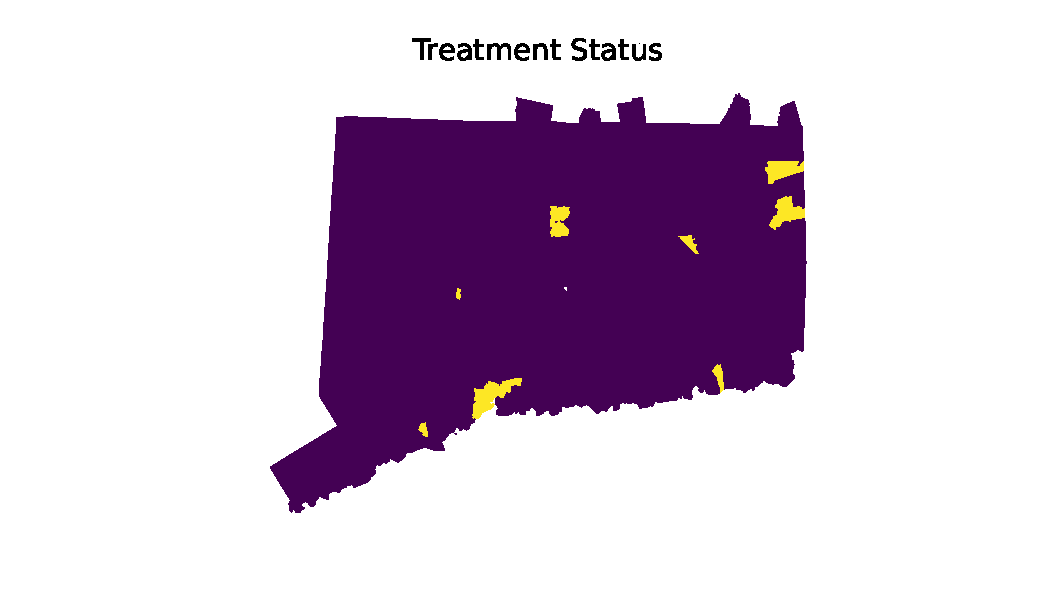
\includegraphics[width=0.5\textwidth]{figures/rtc/maps/zip_code_status.pdf}  
        \caption{Treatment status for each zip code (yellow indicates treated zip code): \href{https://github.com/pharringtonp19/evictions/blob/main/scripts/joint/maps/treatment_status.py}{Reproduced Here}}
\end{figure}

\subsection{Data \& Outcomes}
As referenced prior, the outcome of interest is the search length for households who are currently experiencing homelessness but face limited barriers to housing. Rapid Re-housing, a federally tracked program, provides limited short term assistance to exactly this population. Its aim is to help ``families exit shelters and get back into permanent housing quickly.''\footnote{\textrm{Missing Source}} While different in nature than an independent housing search, the search length of individuals in a Rapid Rehousing program a reasonable proxy for the following three reasons. First, Rapid Rehousing programs ``serve people experiencing homelessness with no preconditions such as employment, income, absence of criminal record, or sobriety.''\footnote{\href{https://www.urban.org/sites/default/files/publication/99153/rapid_re-housings_role_in_responding_to_homelessness_3.pdf}{Reference}} Second, the program does not target people who might need long-term assistance. Those individuals and families are helped by permanent supportive housing programs.\footnote{Very different from permanent supportive housing which is as Rosanne Haggerty writes in the NyTimes, ``is ideal for those with serious health challenges who have been homeless for long periods of time''.\footnote{\href{https://www.nytimes.com/roomfordebate/2015/02/19/homes-for-the-homeless/for-even-the-neediest-housing-is-the-solution-to-homelessness}{NyTimes}}}\footnote{ \textbf{Cost}: at $\$6,678$ per family, it is cheaper than transitional housing at $\$32,557$ per family.\footnote{\href{https://cceh.org/provider-resources/rapid-rehousing/}{CCEH Video}}} Third, the lease agreement households sign come with ``the same rights and responsibilities as a typical lease holder.''\footnote{\href{thttps://endhomelessness.org/resource/rapid-re-housing-a-history-and-core-components/}{It} is imperative that any lease agreement provides the tenant with **the same rights and responsibilities as a typical lease holder** and that the financial terms of the lease are such that the household has a reasonable ability to assume rental costs once financial support ends (keeping in mind that in the majority of cases, even households with no income at move-in retain their housing)"}
\begin{figure}[htbp]
\centering
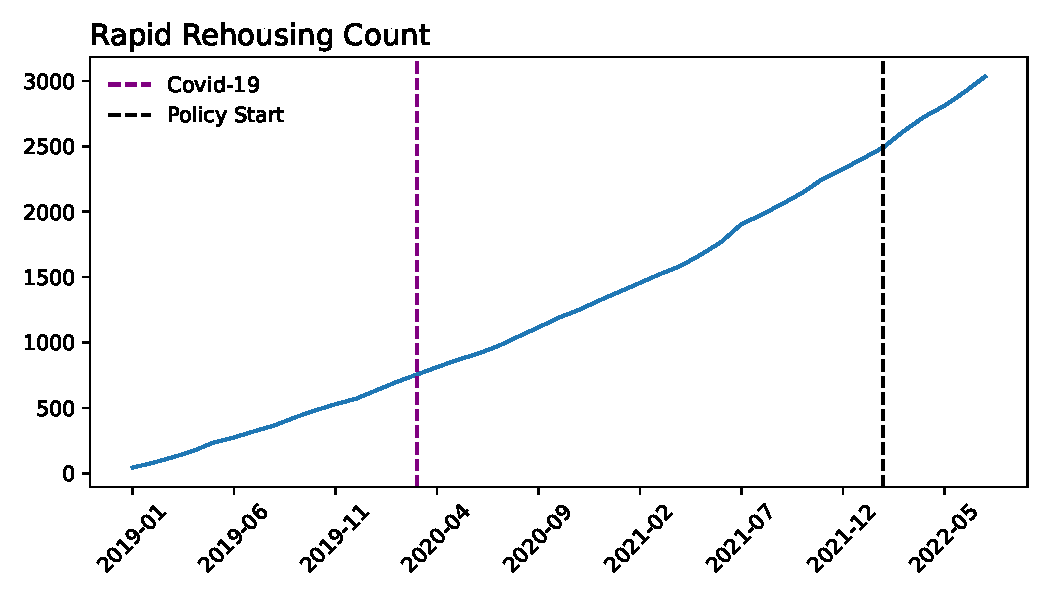
\includegraphics[width=0.5\textwidth]{figures/rtc/context/rrh_counts.pdf}
        \caption{Treatment status for each zip code (yellow indicates treated zip code): \href{https://github.com/pharringtonp19/evictions/blob/main/scripts/cceh/plot/summary_rrh.py}{Reproduced Here}}
\end{figure}

\section{Empirical Strategy}
In contrast to many applied microeconomic papers that assess the sensitivity of their results by varying the selection of the controls in their regression models, we follow the framework presented in our accompanying paper \href{https://github.com/pharringtonp19/rfp_paper/blob/main/Regularizing_the_Forward_Pass.pdf}{Regularizing the Forward Pass} which keeps the set of controls fixed and explores how the estimate varies as we expand the function space that we search over.\footnote{If you are familiar with our ongoing work, you will notice that we have not yet applied the full model in this paper. We plan to do so in the next iteration of the paper.}\par 


The following notation defines the key variables used in the estimators defined below. 
\begin{align*}
    &Y_i: \textrm{Acceptable Move-in Date} \mid \textrm{Search Duration}\\
    &X_i: \textrm{Primary Controls: Age, Gender, Race, Family Size}\\ 
    %&P_i: \textrm{Rapid Rehousing Provider}\\ 
    &Z_i: \textrm{Zip Code} \\
    &D_i: \textrm{Treated Zip Code}
\end{align*}
\textbf{Note}: Subscripts on the outcome corresponding to subsets of individuals who are observed in that corresponding time period. 

\subsection{Difference-in-Difference}
We fit the following difference-in-difference estimator. 
\begin{align*}
    \beta_0 &= \mathbb{E}[Y_1 -Y_0 \mid D=1] -  \mathbb{E}[Y_1 - Y_0 \mid D=0] \end{align*}
    
\begin{figure}[htbp]
\centering
\begin{subfigure}{.48\textwidth}
    \centering
    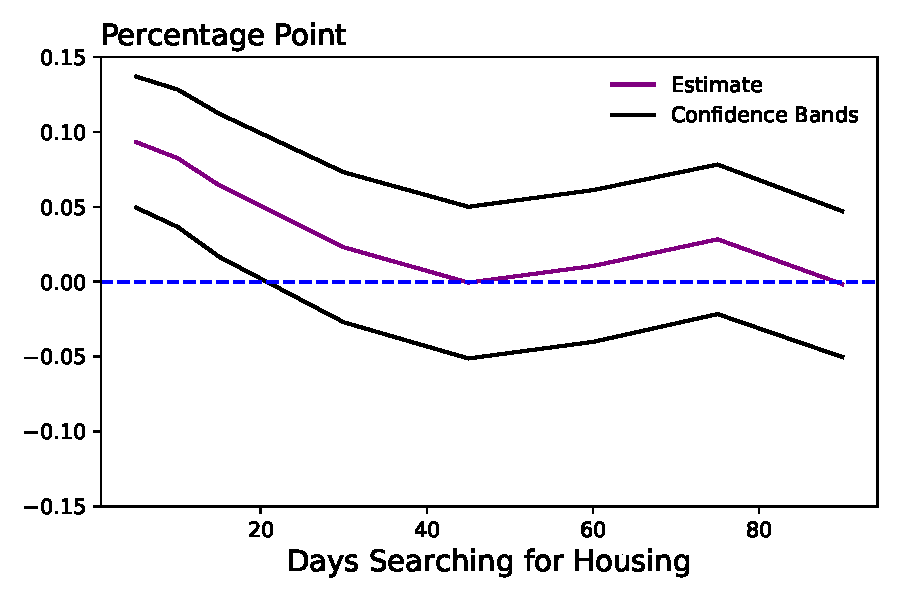
\includegraphics[width=.95\linewidth]{figures/rtc/results/cceh/diff_in_mean_False.pdf}
    \caption{All zip codes}
    \label{SUBFIGURE LABEL 3}
\end{subfigure}
\begin{subfigure}{.48\textwidth}
    \centering
    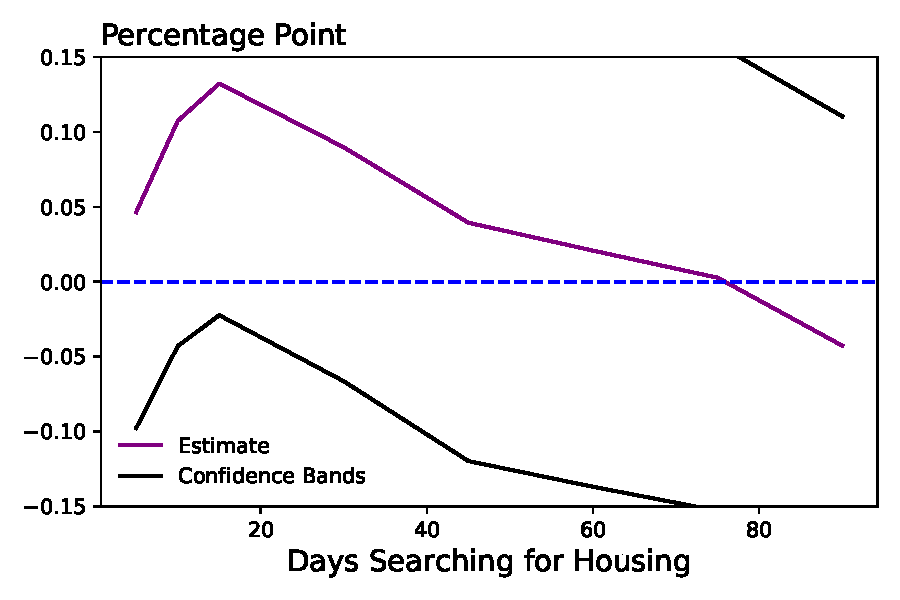
\includegraphics[width=.95\linewidth]{figures/rtc/results/cceh/diff_in_mean_True.pdf}
    \caption{High Eviction Zip Codes}
    \label{SUBFIGURE LABEL 4}
\end{subfigure}
\caption{ \href{https://github.com/pharringtonp19/evictions/blob/main/scripts/cceh/primary/diff_n_mean_rrh.py}{Reproduced Here}: Confidence Bands formed via stratified bootstrapped sampling without replacement (75\%)}
\label{FIGURE LABEL}
\end{figure}

\subsection{Difference-in-Difference with Controls}
We then add individual level and zip code controls to the regression specification
\begin{align*}
    Y_i &= \alpha _0 + \beta_0 \textrm{Post}_i \times \textrm{Treated}_i + \beta_1  \textrm{Post}_i + \beta_2 \textrm{Treated}_i \\ 
    &\quad + \beta _3X_i + \beta_4 Z_i + \varepsilon_i
\end{align*}
\begin{figure}[htbp]
\centering
\begin{subfigure}{.48\textwidth}
    \centering
    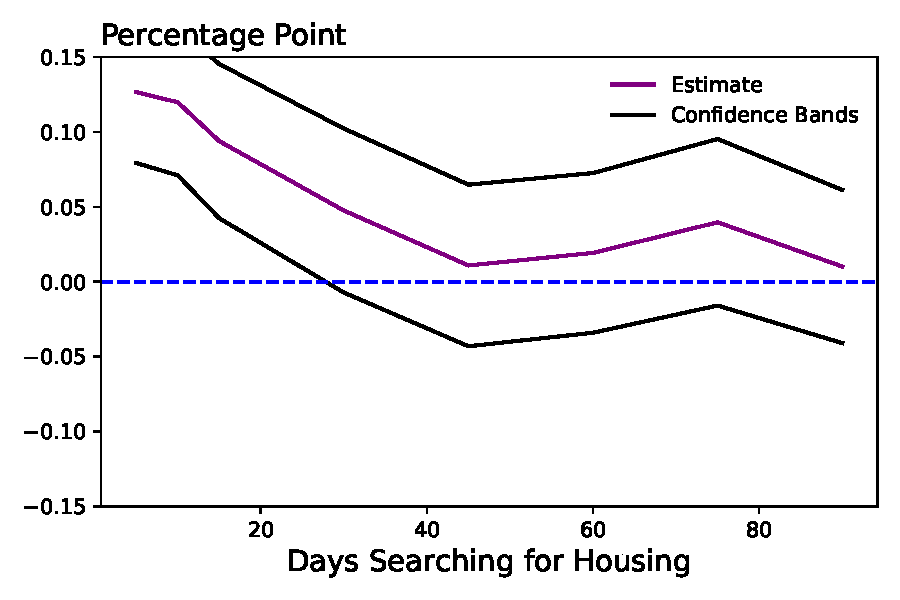
\includegraphics[width=.95\linewidth]{figures/rtc/results/cceh/linear_reg_False.pdf}
    \caption{All zip codes}
    \label{SUBFIGURE LABEL 3}
\end{subfigure}
\begin{subfigure}{.48\textwidth}
    \centering
    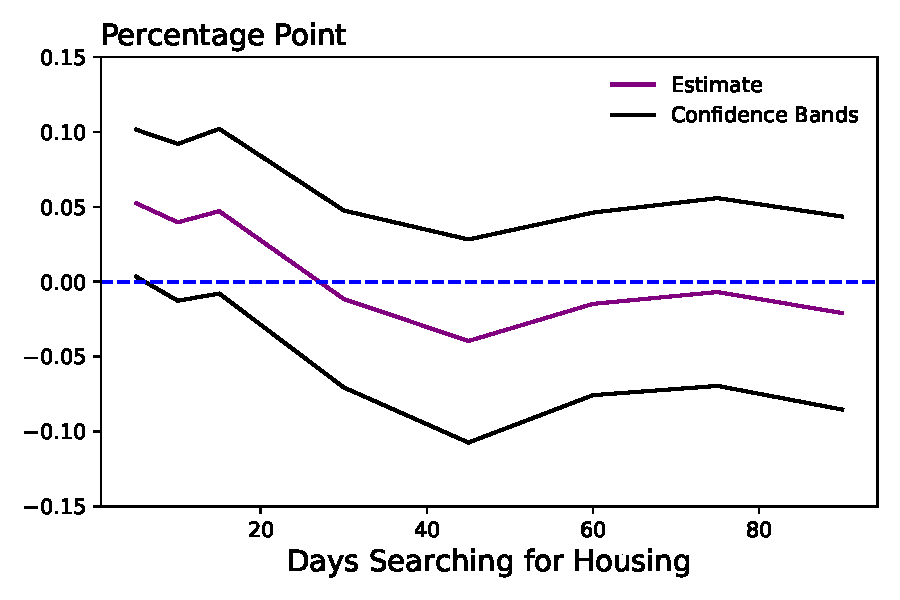
\includegraphics[width=.95\linewidth]{figures/rtc/results/cceh/linear_reg_True.pdf}
    \caption{High Eviction Zip Codes}
    \label{SUBFIGURE LABEL 4}
\end{subfigure}
\caption{ \href{https://github.com/pharringtonp19/evictions/blob/main/scripts/cceh/primary/diff_n_mean_rrh.py}{Reproduced Here}: Confidence Bands formed via stratified bootstrapped sampling without replacement (75\%)}
\label{FIGURE LABEL}
\end{figure}

\subsection{Partially Linear Difference-in-Difference}
As suggested by the explicit functional form, the above estimator doesn't have a non-parametric analogue which may make the interpretation suspect or difficult to some.\footnote{To be clear about this point, it's not obvious how to interpret the coefficient of interest as the result of regression residuals on residuals in the spirit of via Frisch-Waugh-Lovell. That is, the estimator does not have the following nonparametric equivalent: 
\begin{align*}
    Y_i - f_{\theta _1}(Y_i) = \beta_0 (D_i-f_{\theta _2}(D_i)) + \varepsilon_i
\end{align*}}
The natural extension to the difference-in-difference estimator such that it has a Frisch-Waugh-Lovell type of interpretation is the following model where we approximate the conditional expectations via neural network-based estimators.

\begin{itemize}
  \item In the post period, $\mathbb{P}_X,\mathbb{P}_{Y|X}$ might differ because of time and because of the policy
\end{itemize}
\begin{align*}
    Y_{1} - \mathbb{E}[Y_{0} | X_i] &= \beta _0 \big(D_i - \mathbb{E}[D_1 | X_1]\big) + \varepsilon_i
\end{align*}
\subsection{Nonparametric Difference-in-Difference}
A drawback of the above approach is that it makes no correction for the propensity score. 

\begin{align*}
    \beta _0 = \int d\mathbb{P}_X\Big(\big(\mathbb{E}[Y_1 |X,D=1] - \mathbb{E}[Y_0 |X,D=1]\big) -  \big(\mathbb{E}[Y_1 |X,D=0] - \mathbb{E}[Y_0 |X,D=0]\big)\Big)
\end{align*}

\section{Related Literature}
 While this paper certainly engages with various literatures, from statistical discrimination, to applied deep learning, its central aim is to provide additional insight into the effectiveness of the Right to Counsel. \par 
 In line with the recent Economic works on the topic, it does so by offering a partial assessment of the policy ``at scale''. This approach differs significantly from some of the prior randomized control trial studies where only a limited number of judges were involved as in \cite{greiner2012limits} or where only individuals who were thought to likely benefit from legal representation were provided with laywers from private firms working pro bono as in \cite{seron2001impact}.   

In contrast to the recent Economic literature, though, this paper empirically considers the indirect effects of the policy, thereby complementing \cite{cassidy2022effects} which empirically focuses on the direct effects, and \cite{abramson2021welfare} which considers the indirect effects via a counterfactual exercise.
\section{Conclusion}
As a general statement, Economists are interested in understanding the effects of policies at scale. Almost by definition, though, these effects are not well identified.\footnote{The example of cross-country regression highlights this lack of identification} Therefore, the aim is often to capture a particular effect of the policy as it's in the process of being deployed at scale with the hope that this intermediate measurement might be informative about the effects of the policy under the new equilibrium.\par 
In this paper, where we're interested in studying the effects of the Right to Counsel at scale, we take as our intermediate measurement the length of the housing search process for low-income individuals. The thinking being that if there are adverse effects of this policy, that is, if landlords decide to reoptimize in response to the implicit higher eviction costs that the Right to Counsel places on them, we would see it via the housing search channel. \par 
And indeed, while extremely preliminary, we see some indication that there may be adverse effects along this channel. While noisy the estimates suggest that the policy may make it more difficult on average to find housing and in particular for African American women. We caution, though, that our results are preliminary. 

%\bibliographystyle{plainnat}
\bibliography{bibliography.bib}
\end{document} 

